\section{Date: 2024-12-15}
\noindent \textbf{Series ID: COASEANZ11} 

\noindent This series is titled Import Price Index: Agriculture, forestry, fishing and hunting for Association of Southeast Asian Nations (DISCONTINUED) and has a frequency of Monthly. The units are Index 2010=100 and the seasonal adjustment is Not Seasonally Adjusted.The observation start date is 2012-06-01 and the observation end date is 2016-12-01.The popularity of this series is 1. \\ 

\noindent \textbf{Series ID: USUKFXUKM} 

\noindent This series is titled U.S. / U.K. Foreign Exchange Rate in the United Kingdom and has a frequency of Monthly. The units are U.S. Dollars to One British Pound and the seasonal adjustment is Not Seasonally Adjusted.The observation start date is 1791-01-01 and the observation end date is 2017-01-01.The popularity of this series is 23. \\ 

\subsection{Regression Tables and Plots}
\begin{center}
\begin{tabular}{lclc}
\toprule
\textbf{Dep. Variable:}          & value\_fred\_USUKFXUKM & \textbf{  R-squared:         } &     0.276   \\
\textbf{Model:}                  &          OLS           & \textbf{  Adj. R-squared:    } &     0.262   \\
\textbf{Method:}                 &     Least Squares      & \textbf{  F-statistic:       } &     20.18   \\
\textbf{Date:}                   &    Sun, 15 Dec 2024    & \textbf{  Prob (F-statistic):} &  3.85e-05   \\
\textbf{Time:}                   &        22:00:37        & \textbf{  Log-Likelihood:    } &    50.428   \\
\textbf{No. Observations:}       &             55         & \textbf{  AIC:               } &    -96.86   \\
\textbf{Df Residuals:}           &             53         & \textbf{  BIC:               } &    -92.84   \\
\textbf{Df Model:}               &              1         & \textbf{                     } &             \\
\textbf{Covariance Type:}        &       nonrobust        & \textbf{                     } &             \\
\bottomrule
\end{tabular}
\begin{tabular}{lcccccc}
                                 & \textbf{coef} & \textbf{std err} & \textbf{t} & \textbf{P$> |$t$|$} & \textbf{[0.025} & \textbf{0.975]}  \\
\midrule
\textbf{const}                   &       0.9622  &        0.128     &     7.541  &         0.000        &        0.706    &        1.218     \\
\textbf{value\_fred\_COASEANZ11} &       0.0064  &        0.001     &     4.492  &         0.000        &        0.004    &        0.009     \\
\bottomrule
\end{tabular}
\begin{tabular}{lclc}
\textbf{Omnibus:}       & 16.564 & \textbf{  Durbin-Watson:     } &    0.107  \\
\textbf{Prob(Omnibus):} &  0.000 & \textbf{  Jarque-Bera (JB):  } &   19.668  \\
\textbf{Skew:}          & -1.222 & \textbf{  Prob(JB):          } & 5.36e-05  \\
\textbf{Kurtosis:}      &  4.615 & \textbf{  Cond. No.          } &     861.  \\
\bottomrule
\end{tabular}
%\caption{OLS Regression Results}
\end{center}

Notes: \newline
 [1] Standard Errors assume that the covariance matrix of the errors is correctly specified.

\begin{figure}
\centering
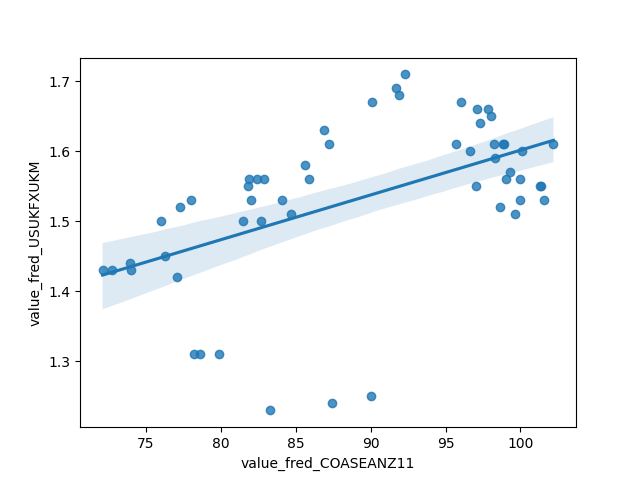
\includegraphics[scale = 0.9]{plots/plot_2024-12-15.png}
\caption{Regression Plot for 2024-12-15}
\end{figure}
\newpage
